\documentclass[main.tex]{subfiles}

\begin{document}
\subsubsection{Submission overview}
For the project, you will be submitting the following:
\begin{enumerate}
\item Zoomed-out photo of Moon in daytime
\item Zoomed-in photo of Moon, taken at same time
\item Zoomed-in photo of golf ball model Moon from scale distance
\item Stellarium screenshot
\item Project report
\end{enumerate}

\subsubsection{Moon photos}
For this project, get a photo of the Moon during the daytime. You can do this from anywhere, and take two pictures at one time.
\begin{enumerate}
\item Take one photo zoomed-out as much as possible (but not past zoom 1$\times$, same as for the sunset photos project), showing both the horizon and the Moon visible. (The Moon will look very small in this picture.)
\item Take a second picture zoomed-in as much as possible on the Moon, at the same time (i.e. right before or after the zoomed-out photo).
\end{enumerate}

Reference Fig.~\ref{fig:moonphot} for an idea of what the photos might look like.

\begin{figure}[htbp]
\begin{center}
	\begin{minipage}{0.3\textwidth}
	\centering
	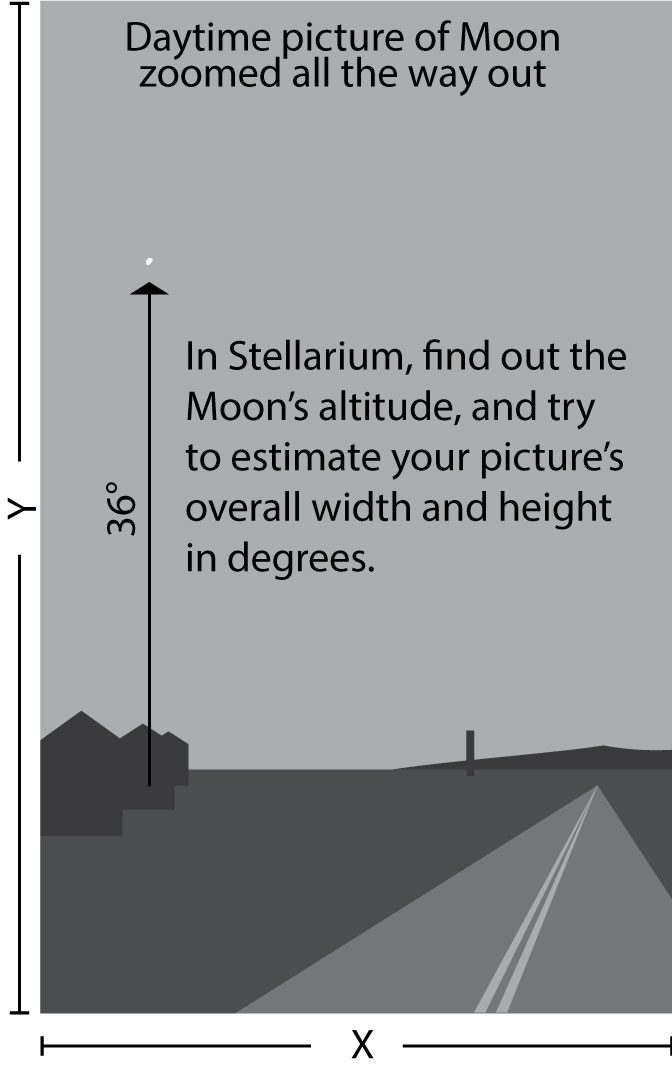
\includegraphics[width=\textwidth]{moonproj_zoomout.jpg}
	%\caption{}
	\end{minipage}
	\begin{minipage}{0.3\textwidth}
	\centering
	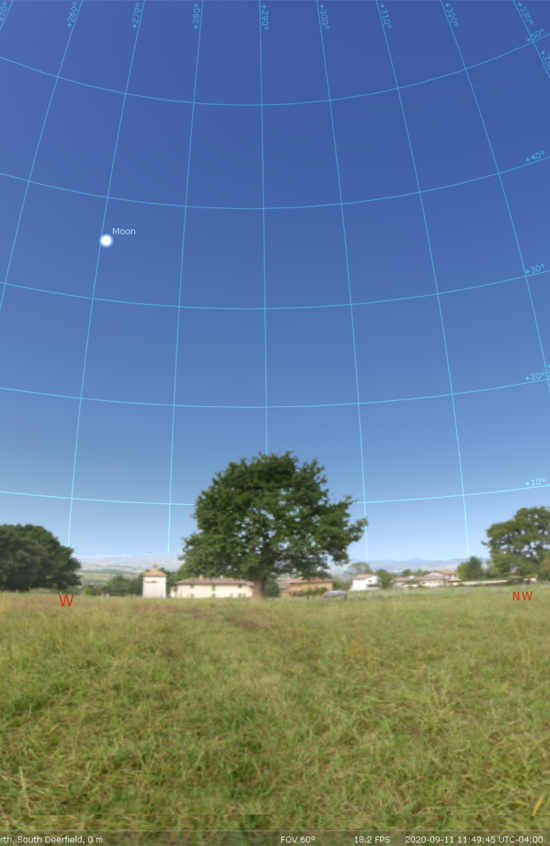
\includegraphics[width=\textwidth]{moonproj_stel.png}
	%\caption{}
    \end{minipage}
	\begin{minipage}{0.3\textwidth}
	\centering
	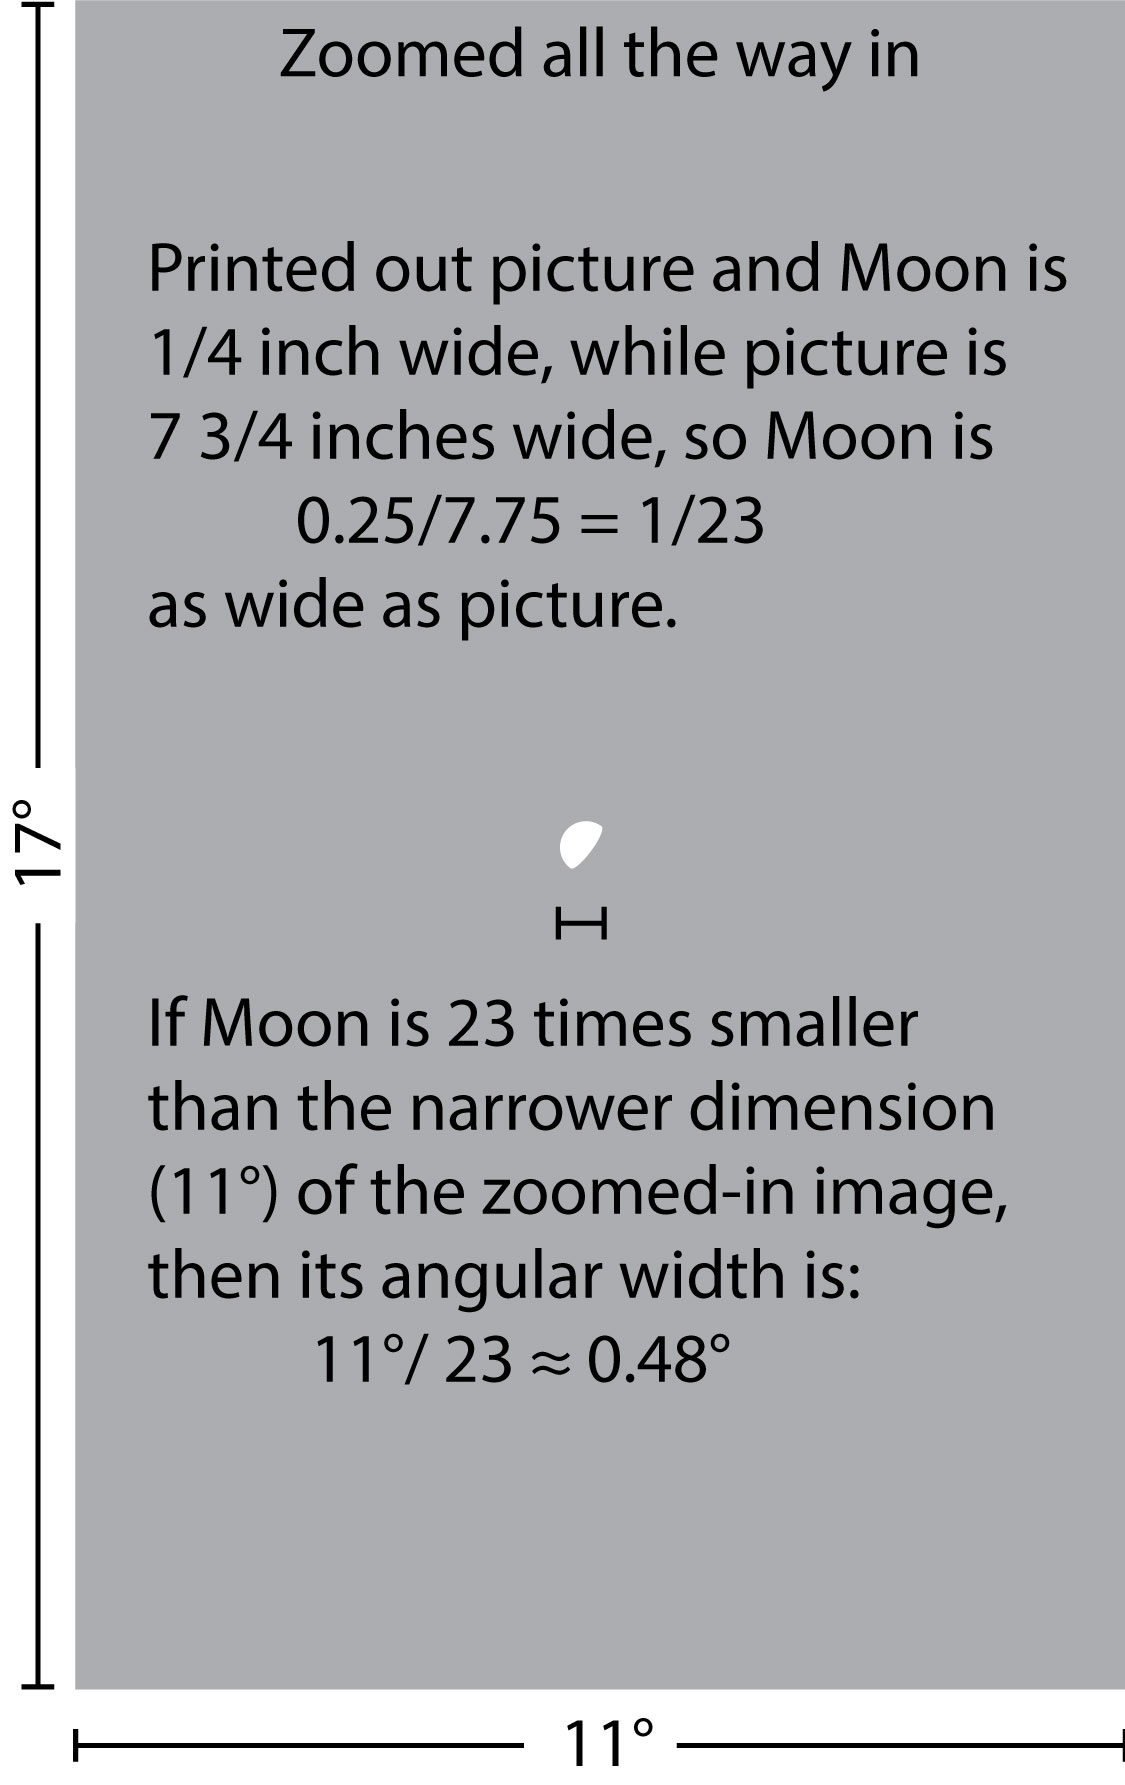
\includegraphics[width=\textwidth]{moonproj_zoomin.jpg}
	%\caption{}
    \end{minipage}
\caption{}
\label{fig:moonphot}
\end{center}
\end{figure}

Submit both the photos as part of the project.

\subsubsection{Model Moon photo}
In Lab~\ref{apx:lab_04}, you will have had a chance to take a fully zoomed-in photo of the golf ball, which we are using to model the Moon, from a to-scale distance. As your camera's zoomed-in angular field of view should be consistent (as long as the camera and zoom settings are the same), the size of the golf ball in this photo should be similar to the size of the actual Moon in your zoomed-in photo of it. If you did not have a chance to do so, let us know so you can make it up.

Submit the photo as part of the write-up portion of the project.

\subsubsection{Stellarium}
Similar to the sunset photos project, take a screenshot of Stellarium set to the same location and time as the zoomed-out photo. Make sure to click on the Moon to show its information. It should look something like what's shown in Fig.~\ref{fig:moonphot} (which unfortunately does not show the information panel that you should include.)

One of the goals of this project is to learn \textbf{when} you can see the Moon during the daytime, and \textbf{where} to look. This changes with the phase of the Moon, and Stellarium can be very helpful in figuring this out.

You can also search on the internet for moonrise and moonset times, and then you work out where the Moon will be as it goes from east to west. You will also have to plan around the weather.

Submit the screenshot as part of the project.

\subsubsection{Project report}
Similar to the sunset photos project, the project report consists of a quiz section and write-up section, both on Moodle. You will not have a submit a separate document for it.

The quiz section will have you enter specifics about your photos, including date, time, azimuth and altitude of the Moon, times of sunrise and sunset, and calibrated angular field of view. The write-up section will ask you to discuss the following:
\begin{enumerate}
\item Compare the altitude of the Moon to the height (in degrees) of your zoomed-out calibration picture. Do these values make sense? Explain how they make sense or what might explain any discrepancy.
\item For the zoomed-in picture, how big is the Moon compared to the width (in degrees) found in your zoomed-in calibration photo? Do you get approximately \SI{0.5}{\degree} for the width of the Moon? Explain how you are making your estimate and/or any problems you had in making the measurement.
\item Place the picture of the golf ball model Moon alongside your zoomed-in photo of the Moon in a document and upload it. Comment in the essay box how similar or different the sizes are in the two photos, and discuss any difficulties.
\end{enumerate}

Note that the 3rd item asks you to upload a separate document containing your photo of the golf ball model Moon and your zoomed-in photo of the actual Moon.

\end{document}